\section*{Maneouver study}
\addcontentsline{toc}{section}{Maneouver study}
The higher the velocity is, the bigger the radius - this is, the greater the increase of altitude - given that the wing's flaps cannot deflect enough nor can support as much force to reduce the radius as to the same menauver for a lower velocity.

Note that the centripetal force follows:
\[
F=\frac{mV^2}{R}
\]
Where \textit{m}, \textit{V} and \textit{R} are the aircraft's mass (in kg), velocity (in m/s) and radius (in m) respectively. \\

The only angles affected are gamma $\gamma$ and mu $\mu$ if performed flawlessly. The former is the angle formed between the \textit{x} axis of the horizontal set and the \textit{x} axis of the wind set, while the latter is the one formed between the \textit{y} axis of the same sets. Note that for the whole maneuver the body set remains consistent with the wind set.\\
Figure \ref{fig:paramEvolution} shows how these change in the different phases of the Immelmann turn\\

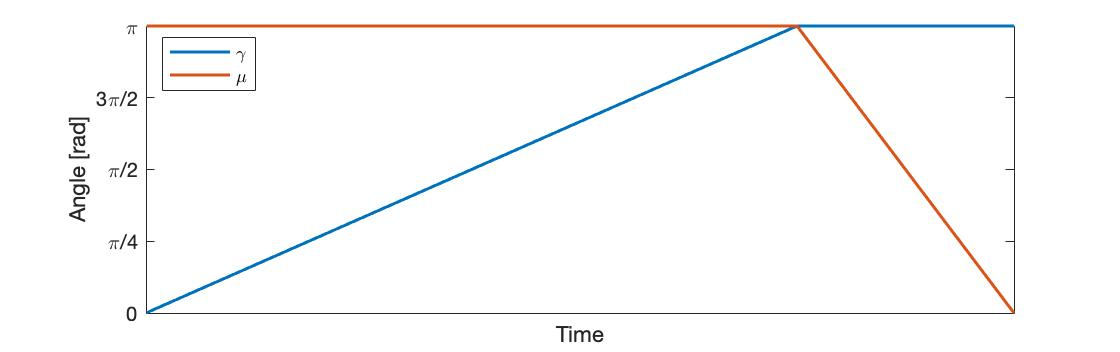
\includegraphics[width=\linewidth]{../matlab/paramEvolution.jpg}
\captionof{figure}{Angles evolution over time}
\label{fig:paramEvolution}
\vspace{0.5cm}

Note that for $\gamma$ the evolution is perfectly defined, as the increment of said angle needs to be positive in order to increase the flight altitude. Conversely, for $\mu$ the pilot could choose to rotate in the opposite direction thus changing $\mu$ from 0 to $-\pi$ instead - note that $\pi$ and $-\pi$ are equivalent -, and the result would be virtually the same.\\
Furthermore, in order to describe a perfect semicircle the angular speed $\dot{\gamma}$ needs to remain constant. This results in the necessary condition of gamma's evolution to be a straight slope. For $\mu$, however, the pilot could also perform the roll at non-constant rotating speed without this having an impact on the maneuver performance. This would be reflected as a curve on mu's temporal evolution, instead of a straight line.

For the following computations, some values will be needed in order to numerically solve the Ordinal Differential Equation systems. The ENAERT T-35 Pillán, a Chilean military small aircraft and its data \cite{jane1969jane} have been taken as references.\\

\begin{center}
	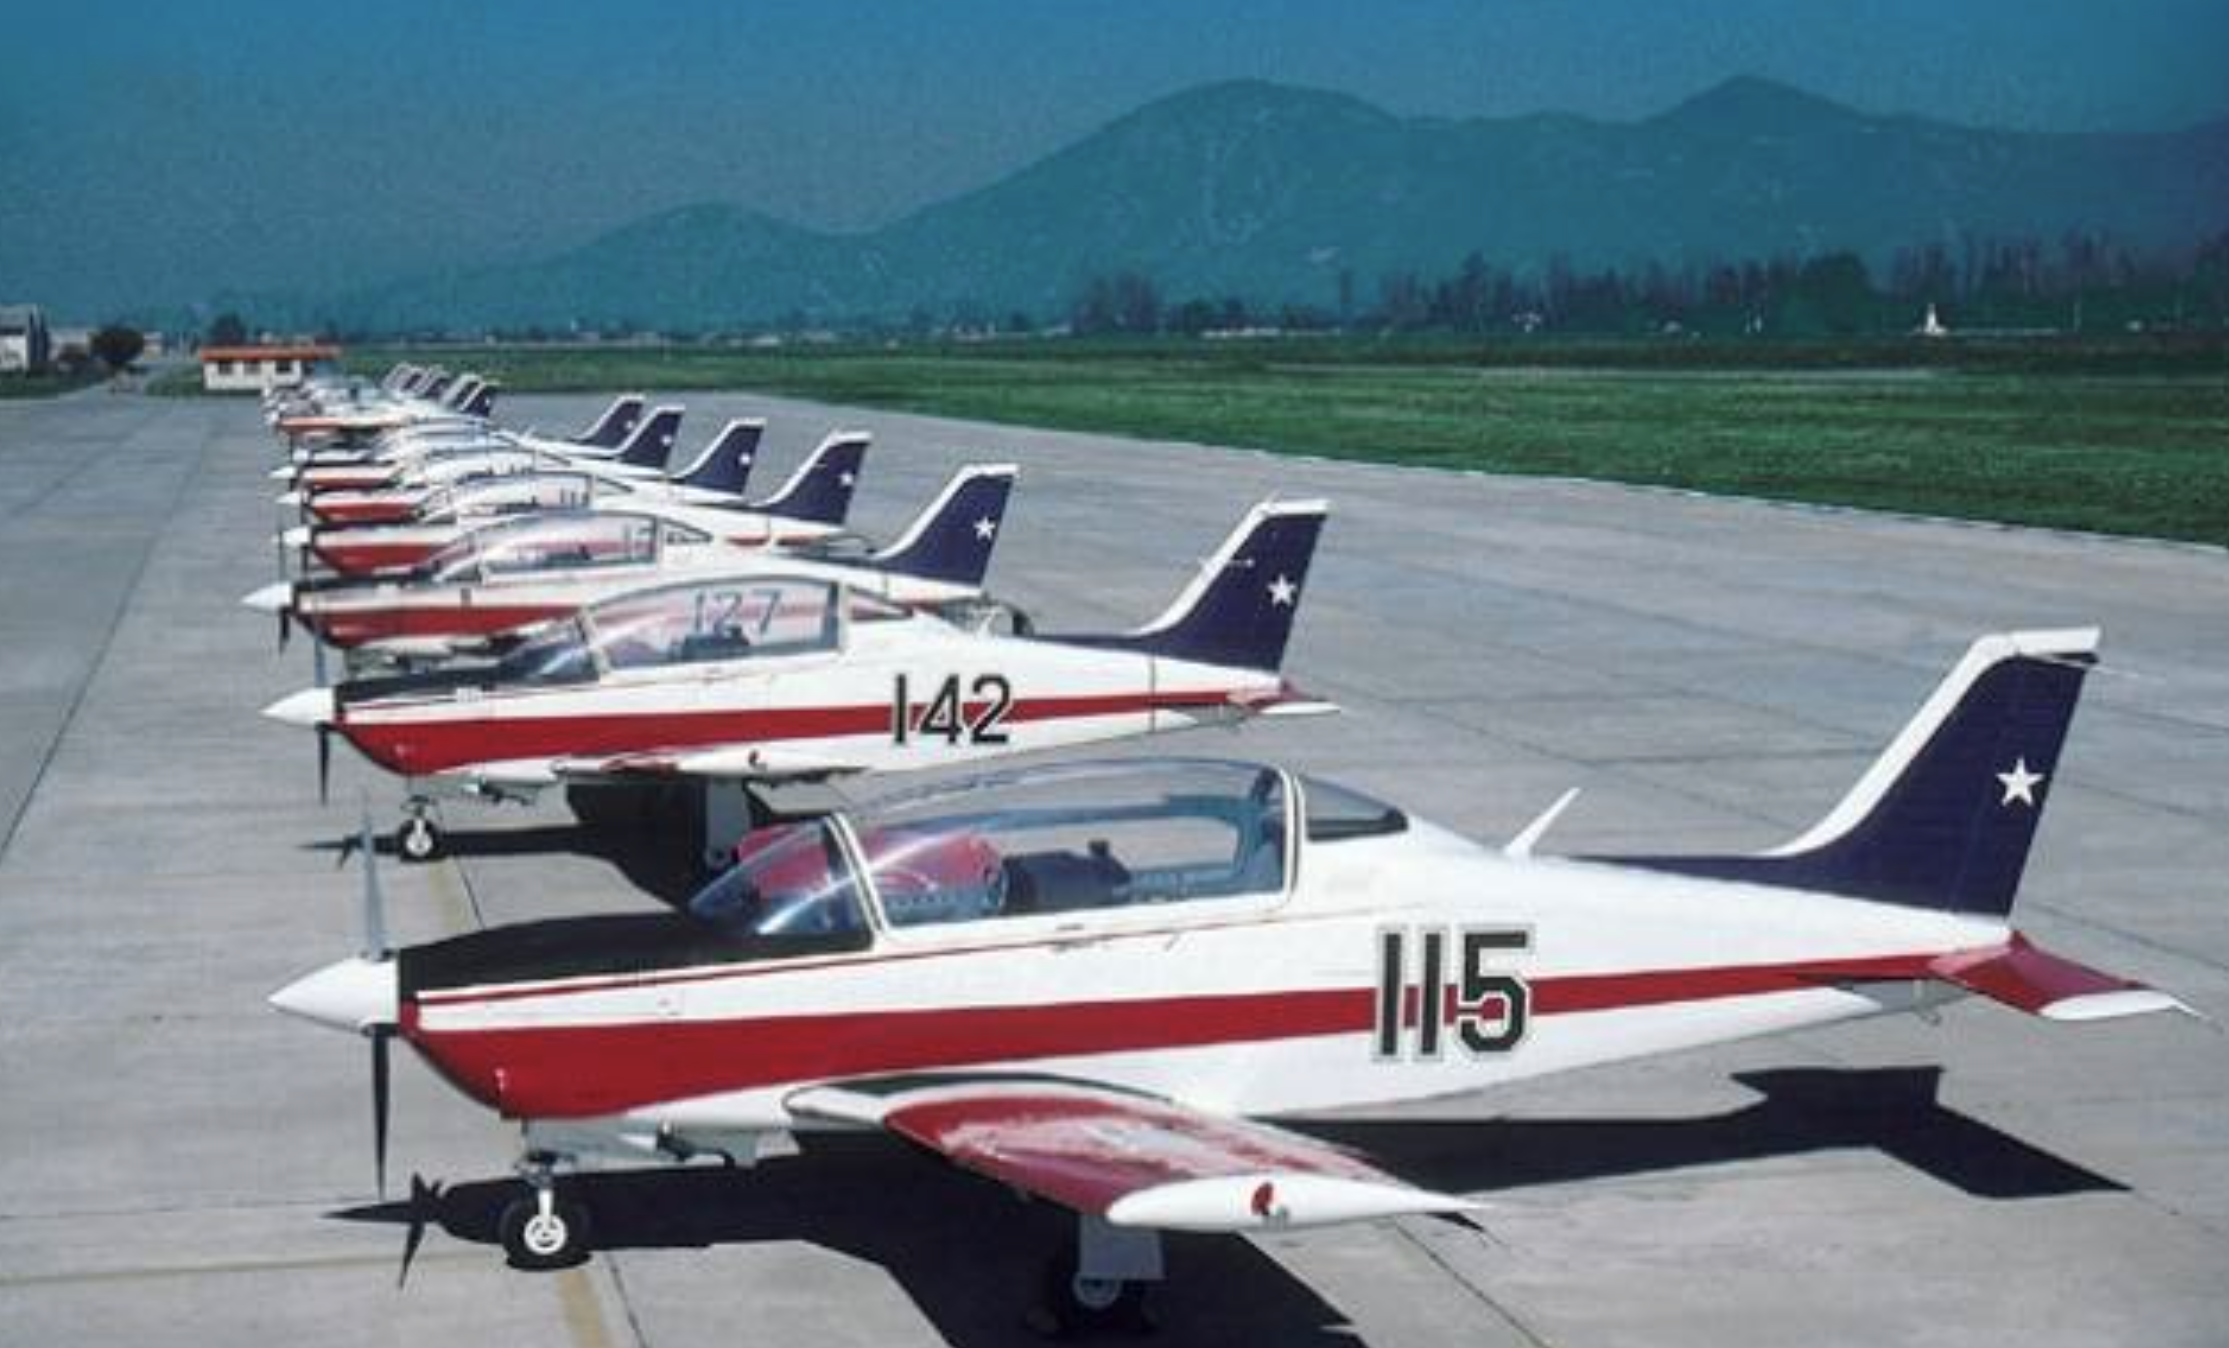
\includegraphics[width=0.9\linewidth]{figures/pillan}
	\vspace{0.5cm}
	\captionof{figure}{ENAERT T-35 Pillán. Extracted from \cite{defensa.com_2018}}\vspace{0.25cm}
\end{center}

The used information is:

\begin{center}
\begin{tabular}{|l|l||l|l|}\hline
	 & Value &   & Value\\ \hline \hline
	Mass & 1.300 kg& Wingspan & 8.84 m\\ \hline
	Airfoil & 63$_3$-414 & Wing area & 13.69 m$^2$ \\ \hline
	Stall s. & &  Cruise s. &\\ \hline
	Thrust &224 kW & Air den. & 1.225 kg/m$^3$ \\ \hline
	\multicolumn{4}{|c|}{$C_L=12\alpha+0.33$}\\ \hline	
\end{tabular}
\end{center}

\subsection*{Evolution throughout time}
For the totality of the maneuver, the fixated parameters are the gas control lever ($\pi$) and the elevator ($\alpha$), which are set as constants at 1.5 kN and 0.3 rad respectively. From the remaining variables, the position coordinates evolution ($\Dot{x}$ and $\Dot{z}$) are always left as dependant in order to be solved by the ODE solver. With the obtained results, the trajectory is plot - see the following section Trajectory analysis, where both of them are studied in moer depth -.

For the first and last phases, both cruise flight, the remaining variable (not counting $\Dot{x}$ and $\Dot{z}$) is velocity (V).\\
Evaluate L, D, V, $\gamma$, z, x

\subsubsection*{Cruise flight}

\subsubsection*{Half loop}
Taking the first equation of each of the phases' systems we can operate to integrate the velocity through time. For the most generic case:
\begin{align*}
	\begin{cases}
	\frac{\partial V}{\partial t}=&\frac{1}{m}\left(T - D -mg\sin\gamma\right)\\
	\frac{\partial \gamma}{\partial t}=&\frac{1}{mV}\left(L-mg\cos\gamma\right)
	\end{cases}
\end{align*}
\begin{align*}
	dt =& \frac{m}{T - D -mg\sin\gamma} dV\\
	\int dt= & \int \frac{m}{T - D -mg\sin\gamma} dV
	\intertext{Subsituting drag's definition,}
	= & \int \frac{m}{T - \frac{1}{2}\rho S V^2 (C_{D_0}+kC_L^2) -mg\sin\gamma} dV
\end{align*}

The three force configurations during the maneuver correspond to the free body diagrams at stages 1, 2 and 3 (see Figure \ref{fig:immelmann-overview}). \vspace{0.5cm}

%\begin{minipage}{\textwidth}
	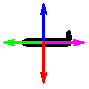
\includegraphics[width=0.3\linewidth]{figures/free-body-1.pdf} \hfill
%	\captionof{subfigure}{Angles evolution over time}
	\label{fig:free-body-1}
		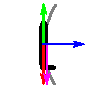
\includegraphics[width=0.3\linewidth]{figures/free-body-2.pdf}\hfill
%	\captionof{subfigure}{Angles evolution over time}
	\label{fig:free-body-2}
		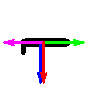
\includegraphics[width=0.3\linewidth]{figures/free-body-3.pdf}
%	\captionof{subfigure}{Angles evolution over time}
	\label{fig:free-body-3}
	\vspace{0.5cm}
	\captionof{figure}{Free body diagrams during the semiloop. Own elaboration.}\vspace{0.25cm}
%\end{minipage}

Note that at all times the lift behaves as the centripetal force, thus indicating that both the velocity and radius limitations to perform the Immelmann turn are inherent to the wing design and its maximum and minimum lift generation.\\
AS the motion will be circular, the normal and tangential accelerations will follow:
\begin{align*}
	a_n=&\frac{V^2}{R}=V\dot{\gamma}=\dot{\gamma}^2R&a_t=V^2R
\end{align*}
As a result, the radius can be writen as a function of the angle of attack. By operating with the third equation of system number \ref{eq:semicircle}, which is in wind system of reference, very convenient as is also polar set of axis:
\begin{align*}
	L=&m\left(\frac{V^2}{R}+g\cos(\gamma)\right)\\
	\frac{1}{2}\rho S V^2 C_L(\alpha)=&m\left(\frac{V^2}{R}+g\cos(\gamma)\right)\\
	R=&\frac{2mV^2}{2W\cos(\gamma)+\rho S V^2 C_L(\alpha)}
\end{align*}
As the plane must describe a semicircle, the radius must be constant.

\begin{center}
	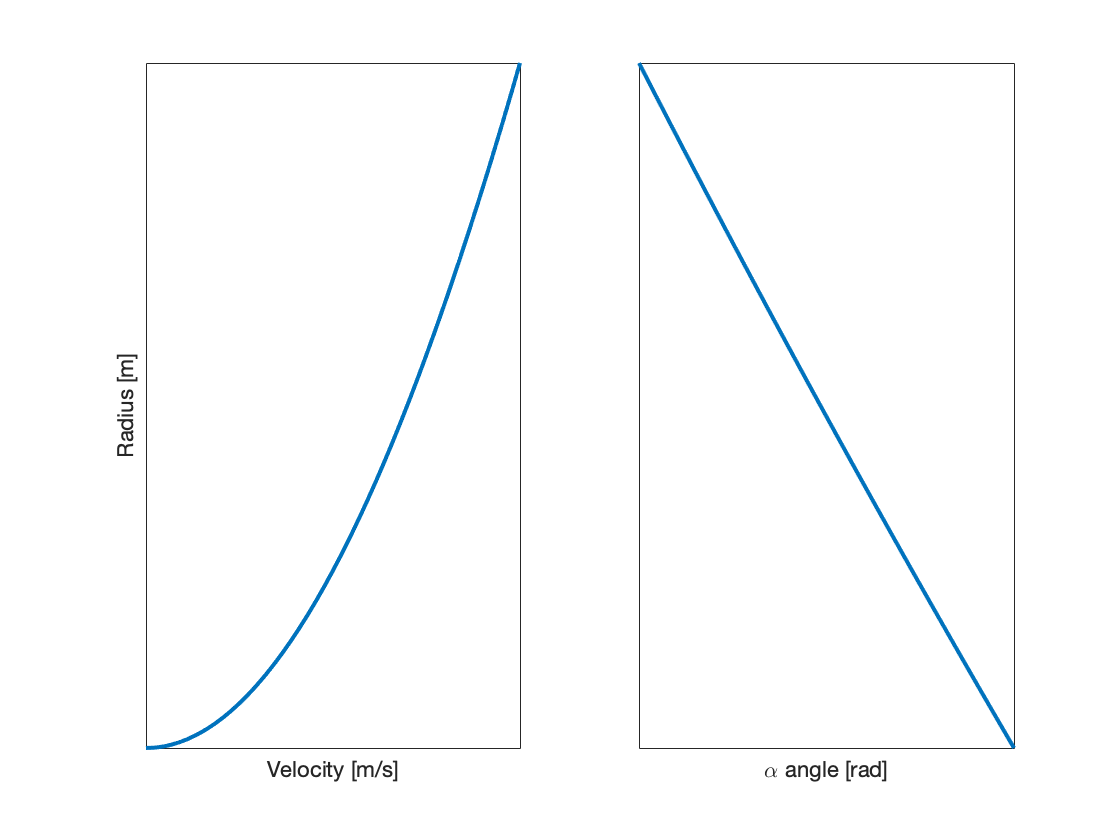
\includegraphics[width=\linewidth]{../matlab/radius.png}
	\vspace{0.5cm}
	\captionof{figure}{Radius dependance on V and $\alpha$t. Own elaboration.}\vspace{0.25cm}
\end{center}

If we take both V (controlled by the gas control lever) and $\gamma$ 
\subsubsection*{Roll}

\subsection*{Trajectory analysis} 
The expected result of the trajectory is portrayed in the following image:

\begin{center}
	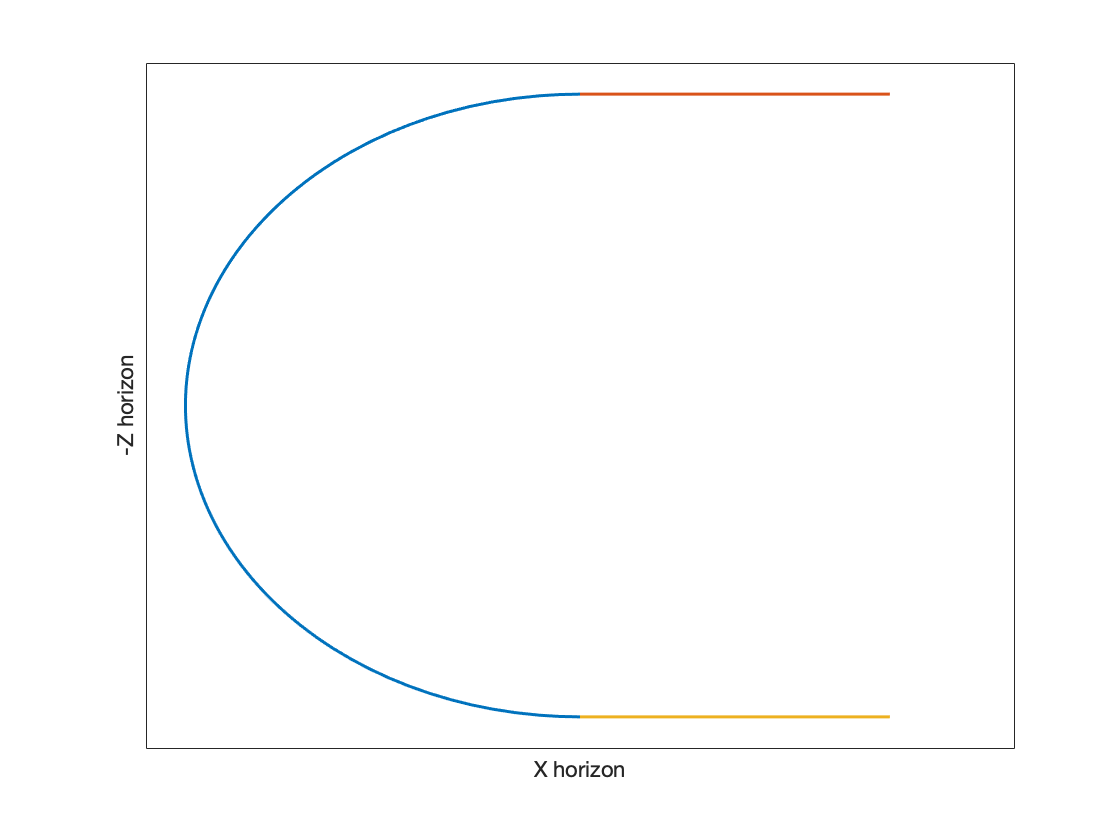
\includegraphics[width=\linewidth]{../matlab/trajectory.png}
	\vspace{0.5cm}
	\captionof{figure}{Expected trajectory output. Own elaboration.}\vspace{0.25cm}
\end{center}

We can consider the maneuver coordinates:
\begin{align*}
	\dot{x}_e=&V\cos\gamma&&&	x_e=&Vt\cos\gamma \\
	\dot{y}_e=&0& \rightarrow&&	y_e=&0\\
	\dot{x}_e=&-V\sin\gamma&&&z_e=&-Vt\sin\gamma
\end{align*}